\section{Istruzioni per l'utilizzo}
\subsection{Autenticazione}

All'avvio verrà mostrata una schermata che servirà ad autenticarsi, bisognerà inserire nome utente e password del proprio account zextras, in caso di successo dell'operazione si avvierà il software, altrimenti verrà visualizzato un messaggio di errore e chiesto di reinserire le credenziali.

\begin{figure}[H]
    \centering
    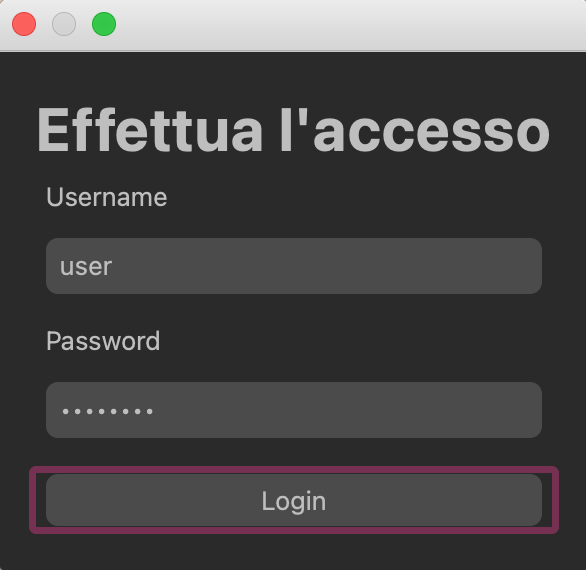
\includegraphics[scale = 0.50]{components/img/login.png}
    \caption{Vista del login}
    \label{fig:Vista del login}
\end{figure}

\subsection{Impostazione del root path}

Al primo avvio dell'applicazione inoltre verrà richiesto di scegliere una cartella, essa sarà la cartella nella quale verranno sincronizzati tutti i file. Non si deve scegliere la stessa cartella nella quale è contenuto il programma.

\subsection{Impostazioni}
\begin{figure}[H]
    \centering
    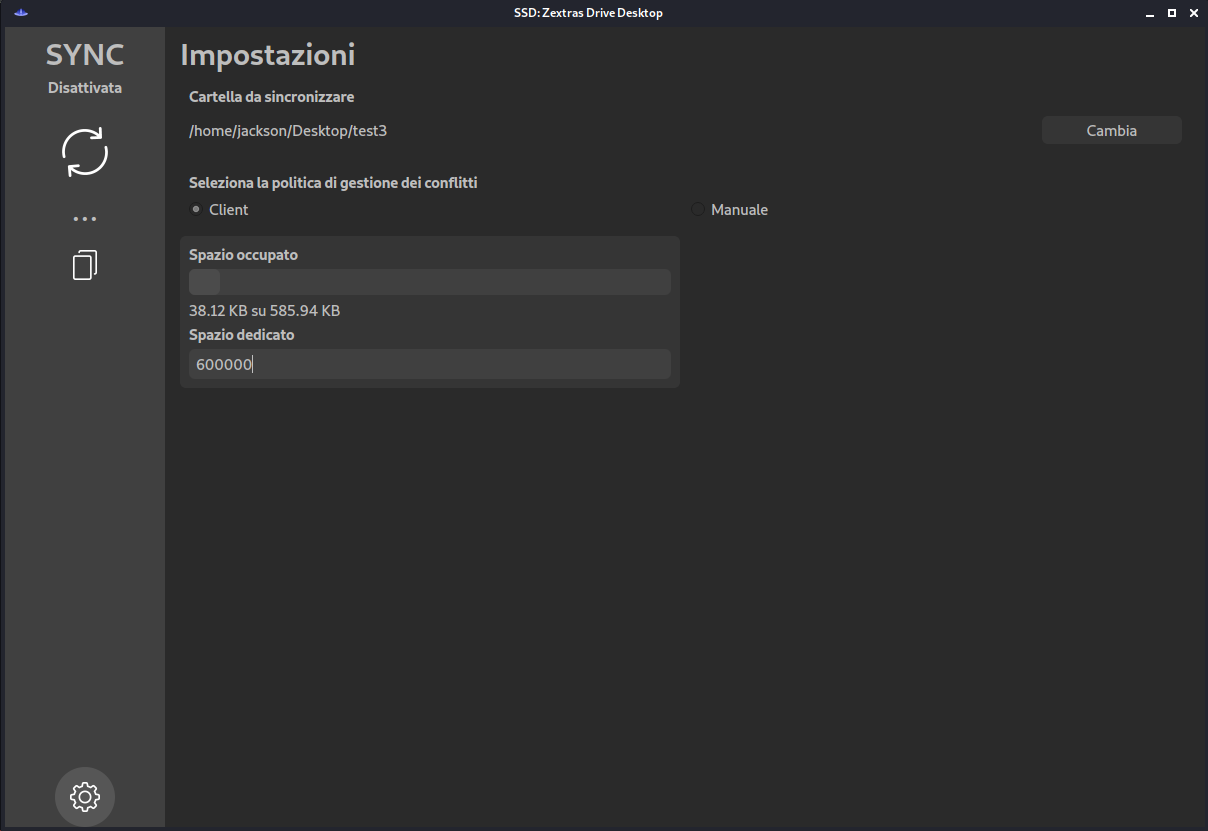
\includegraphics[scale = 0.30]{components/img/settings.png}
    \caption{Vista delle impostazioni}
    \label{fig:Vista delle impostazioni}
\end{figure}


\subsection{Visualizzazione file nel path}

\begin{figure}[H]
    \centering
    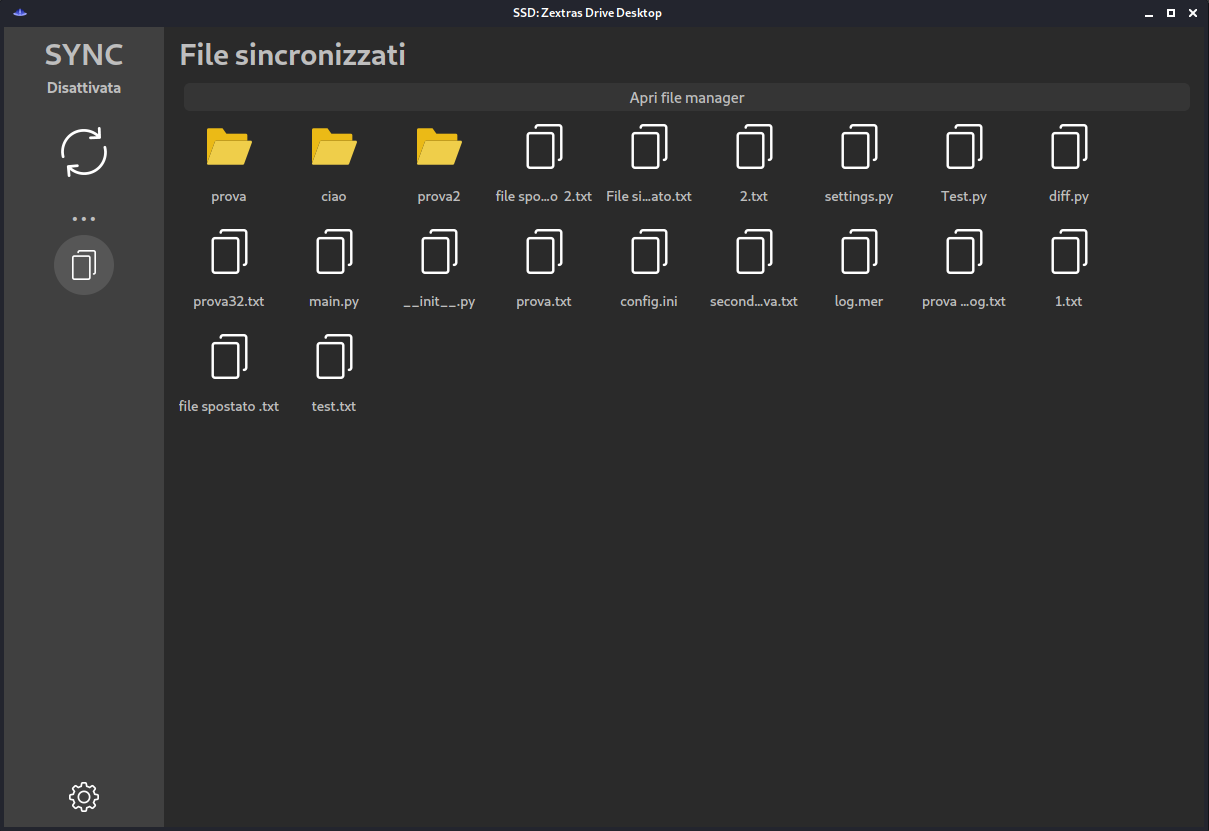
\includegraphics[scale = 0.30]{components/img/file-view.png}
    \caption{Vista dei file nel path}
    \label{fig:Vista dei file nel path}
\end{figure}